\documentclass[12pt,a4paper]{article}
\usepackage{amsmath,amssymb,amsthm,epsf, graphicx, rotating}
\usepackage{fancyhdr}
\usepackage{subfig}
\usepackage{float}
\graphicspath{ {./images/} }

\pagestyle{empty}
\setlength{\parindent}{0pt}
\setlength{\textwidth}{6.5in}
\setlength{\oddsidemargin}{0in}
\addtolength{\textheight}{1in}

\renewcommand\theenumi{\alph{enumi}}
\renewcommand\labelenumi{(\theenumi)}

\newcommand{\Z}{\mathbb{Z}}
\newcommand{\F}{\mathbb{F}}
\newcommand{\R}{\mathbb{R}}
\newcommand{\C}{\mathbb{C}}
\newcommand{\N}{\mathbb{N}}
\renewcommand\vec{\mathbf}

\pagestyle{fancy}
\fancyhf{}
\fancyhead[LE, RO]{Ryan Liu}

\theoremstyle{definition}
\newtheorem{problem}{}

\author{Ryan Liu}
\title{MATH 442 Homework 3}
\begin{document}

\begin{center}
{\huge MATH 442 \par}
{\Large Homework  3  \par}
{\normalsize Name: Ryan Zhuo Lun Liu \par}
{\normalsize Student Number: 30328141 \par}
\end{center}

\begin{problem}
\underline{Answer:} The formula for the number of walks of length $k$ from vertex $A$ to vertex $B$ is: \\

\[
    S(k) =
\begin{cases}
    2^{k - 1},& \text{if } k \text{ is odd} \\
    0,              & \text{otherwise}
\end{cases}
\] \\

\underline{Proof by Induction:} \\
\underline{Base Case:} \\
For $n = 1$, $S(1) = 1$. The adjacency matrix is represented by: \\
\[
A^1 =
\begin{pmatrix}
    0&1&1&0\\
    1&0&0&1\\
    1&0&0&1\\
    0&1&1&0\\
\end{pmatrix}
\] \\

For $n = 2$, $S(2) = 0$. The adjacency matrix is represented by: \\
\[
A^2 =
\begin{pmatrix}
    2&0&0&2\\
    0&2&2&0\\
    0&2&2&0\\
    2&0&0&2\\
\end{pmatrix}
\] \\

From this, we see that the number of walks of length $k$ is defined by the value of the matrix at row 0 and column 1. In addition, we see that the matrices for even and odd $k$ are different and thus we will split the induction into two parts.\\

\underline{Induction Step:} \\
\underline{$k$ is even:} \\
Suppose that $A^k$ = $\begin{pmatrix}
    0&2^{k - 1}&2^{k - 1}&0\\
    2^{k - 1}&0&0&2^{k - 1}\\
    2^{k - 1}&0&0&2^{k - 1}\\
    0&2^{k - 1}&2^{k - 1}&0\\
\end{pmatrix}$  such that $k \geq 1$ \\\\

As $k$ is even, we must prove for $A^{k + 2}$. \\

$A^{k + 2} = (A^k)(A^2)$ =
$\begin{pmatrix}
    0&2^k&2^k&0\\
    2^k&0&0&2^k\\
    0&2^k&2^k&0\\
\end{pmatrix}$
$\begin{pmatrix}
    2&0&0&2\\
    0&2&2&0\\
    0&2&2&0\\
    2&0&0&2\\
\end{pmatrix}$
$= \begin{pmatrix}
    0&2^{k + 1}&2^{k + 1}&0\\
    2^{k + 1}&0&0&2^{k + 1}\\
    2^{k + 1}&0&0&2^{k + 1}\\
    0&2^{k + 1}&2^{k + 1}&0\\
\end{pmatrix}$

\underline{$k$ is odd:} \\
Suppose that $A^k$ = $\begin{pmatrix}
    2^{k - 1}&0&0&2^{k - 1}\\
    0&2^{k - 1}&2^{k - 1}&0\\
    0&2^{k - 1}&2^{k - 1}&0\\
    2^{k - 1}&0&0&2^{k - 1}\\
\end{pmatrix}$  such that $k \geq 1$ \\\\

As $k$ is odd, we must prove for $A^{k + 2}$. \\

$A^{k + 2} = (A^k)(A^2)$ =
$\begin{pmatrix}
    2^k&0&0&2^k\\
    0&2^k&2^k&0\\
    0&2^k&2^k&0\\
    2^k&0&0&2^k\\
\end{pmatrix}$
$\begin{pmatrix}
    2&0&0&2\\
    0&2&2&0\\
    0&2&2&0\\
    2&0&0&2\\
\end{pmatrix}$
$= \begin{pmatrix}
    2^{k + 1}&0&0&2^{k + 1}\\
    0&2^{k + 1}&2^{k + 1}&0\\
    0&2^{k + 1}&2^{k + 1}&0\\
    2^{k + 1}&0&0&2^{k + 1}\\
\end{pmatrix}$

\end{problem}

\begin{problem}
\underline{Answer:} For a graph $G = (V, E)$, each edge has exactly two ends such that each edge will count towards the degree of two vertices. Thus, the sum of the degrees of all the vertices must be even. This statement is true even for loops as the two ends of the edge simply connect to the same vertex. \\

Suppose that the sum of the degrees of all the vertices is even, then there must be an even number of vertices with odd degrees. \\

For any even number $a$ and odd number $b$, it is true that $a$*$a$ is even and that $a$*$b$ is even and that $b$*$b$ is odd. Thus, if the sum of the degrees of all the vertices is even given that some vertices have odd degrees, there must be an even number of vertices with odd degrees.

\end{problem}

\begin{problem}
\underline{Answer:} Yes, it is possible to have a graph with an even number of vertices to have half its vertices of degree $a$ and half its vertices of degree $a + 1$. \\

The condition for a graph with $n$ vertices where $n$ is an even number is that $\frac{n}{2}$ must be an even number as well, meaning that $n \mod 4 = 0$. We first split $n$ vertices into two groups, each with $\frac{n}{2}$ vertices. In order for the statement to be true, each group must be split into two more groups, leaving us with: $A_1, A_2, B_1, B_2$. Creating an additional edge between every vertex in $A_2$ to exactly one vertex in $B_2$ gives us $\frac{n}{2}$ vertices with degree of $a + 1$.

Below is an example of a simple and connected graph with $n = 4$ vertices where two vertices have degree 2 and two vertices have degree 3. \\

\begin{figure}[H]
    \centering
    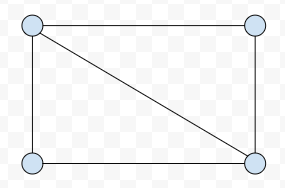
\includegraphics[scale=0.6]{q3.png}
    \caption{Half Vertex Problem}
    \label{fig:my_label}
\end{figure}

\end{problem}

\begin{problem}
\underline{Answer:} \\
Suppose that a simple graph $G = (V, E)$ is self-complementary, then the number of edges in $G$ must be exactly half of all possible edges and the other half belongs to the $G'$. \\

Thus, for a graph $G$ with $n$ vertices, the total number of possible edges is exactly $\frac{n(n - 1)}{2}$. As $G$ is self-complementary, it will have half that, or $\frac{n(n - 1)}{4}$ edges. As $n$ and $n - 1$ cannot both be multiples of 2, $n$ or $n - 1$ must be a multiple of 4, meaning that $G$ must have either $4k$ or $4k + 1$ for some $k$ vertices. \\

An example with 8 vertices is shown in figures 2 and 3. The labels for the vertices have a direct mapping ($A \rightarrow A)$.

\begin{figure}[H]
    \centering
    \begin{minipage}{0.5\textwidth}
        \centering
        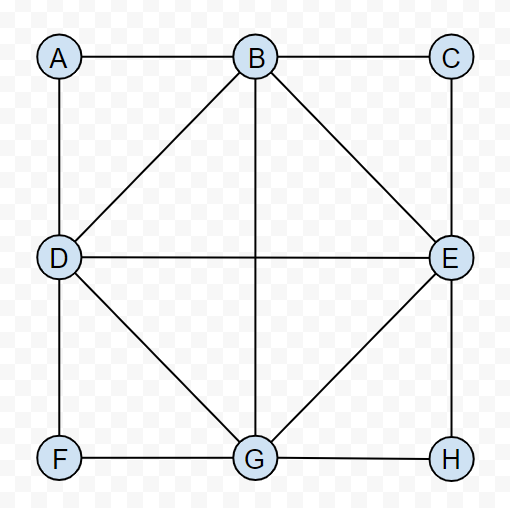
\includegraphics[width=0.9\textwidth]{q4a.png} % first figure itself
        \caption{Graph A}
    \end{minipage}\hfill
    \begin{minipage}{0.5\textwidth}
        \centering
        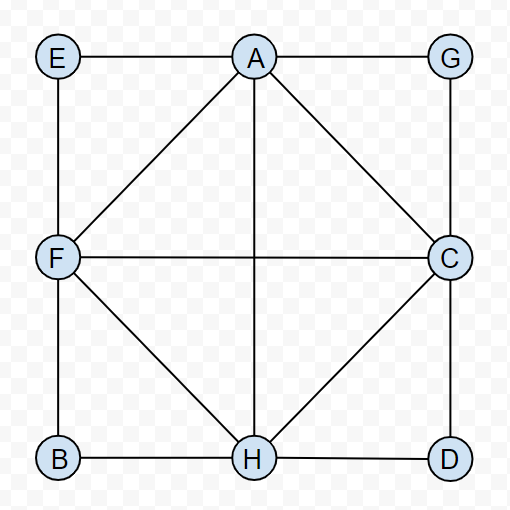
\includegraphics[width=0.9\textwidth]{q4b.png} % second figure itself
        \caption{Complement of A}
    \end{minipage}
\end{figure}

\end{problem}

\begin{problem}
\underline{Answer:} Refer to figures 4 and 5 for all possibilities of graphs for graphs with 2 or 3 vertices. From it, we can see that no graphs with 2 or 3 vertices can be self-complementary.

\begin{figure}[H]
    \centering
    \begin{minipage}{0.5\textwidth}
        \centering
        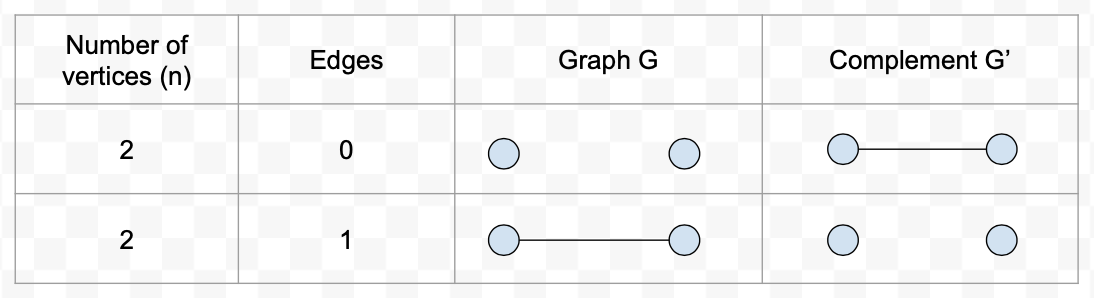
\includegraphics[width=0.9\textwidth]{q5a.png} % first figure itself
        \caption{Graph A}
    \end{minipage}\hfill
    \begin{minipage}{0.5\textwidth}
        \centering
        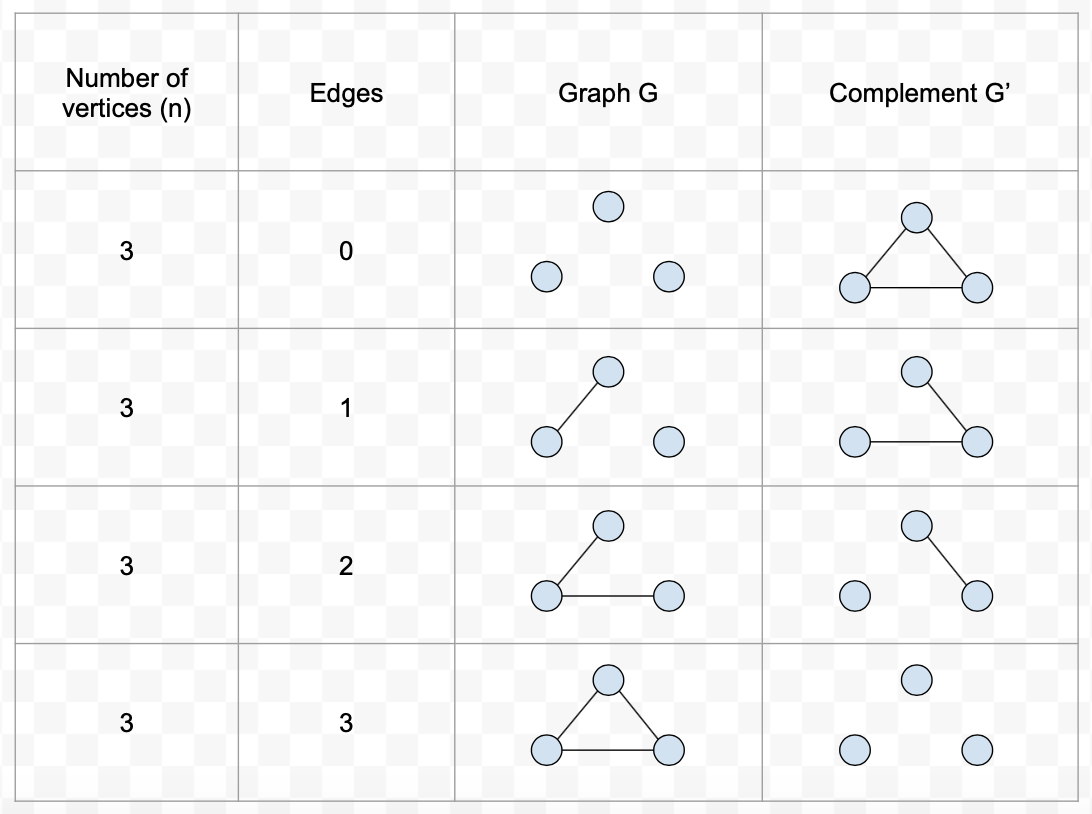
\includegraphics[width=0.9\textwidth]{q5b.png} % second figure itself
        \caption{Complement of A}
    \end{minipage}
\end{figure}
\end{problem}

\begin{problem}
\underline{Answer:} \\
\begin{figure}[H]
    \centering
    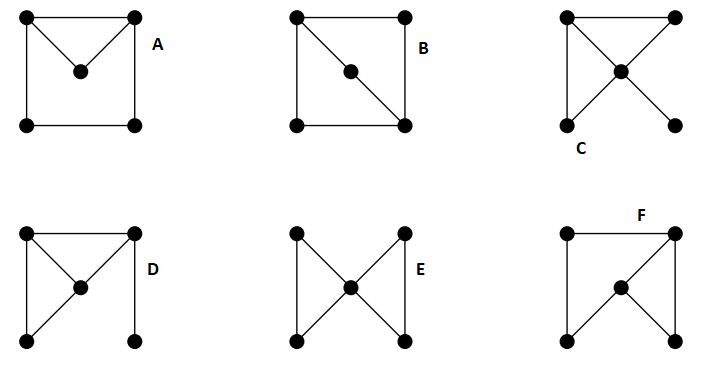
\includegraphics[scale=0.6]{q6.png}
    \caption{Graph Isomorphism Problem}
    \label{fig:my_label}
\end{figure}

Graph A has 3 vertices of degree 2 and 2 vertices of degree 3. \\
Graph B has 3 vertices of degree 2 and 2 vertices of degree 3. \\
Graph C has 1 vertex of degree 1, 2 vertices of degree 2, and 1 vertex of degree 3 and 4. \\
Graph D has 1 vertex of degree 1, 1 vertex of degree 2, and 3 vertices of degree 3\\
Graph E has 4 vertices of degree 2 and one vertex of degree 4. \\
Graph F has 3 vertices of degree 2 and 2 vertices of degree 3. \\

Graphs A and F are isomorphic.

\end{problem}

\begin{problem}
\underline{Answer:} Given that the sequence is of length $k$ ...\\
\underline{The number of vertices for $Q_k$ is $2^k$.} \\

Each sequence is of length $k$ and each number in the sequence can be a 0 or 1, then the total number of possible different sequences is $2^k$. Another way of thinking is that each number has two possibilities, and there are $k$ numbers, then the total number of possibilities must be $2*2*2*2....2 = 2^k$ different sequences. Thus, there are exactly $2^k$ vertices (sequences). \\

\underline{The number of edges for $Q_k$ is $(k)2^{k - 1}$} \\

Suppose that the total number of vertices in such a graph is $2^k$, and that edges exist between vertices whose sequences that differ in just one place. \\

Thus, for each vertex, there are exactly $k$ different ways to modify the sequence such that two sequences differ in one place. Thus, the total number of edges is $(k)2^k$. \\

However, we have to divide by 2 as such a way of counting counts both ends of the edge, meaning the total number of edges is $(k)2^{k - 1}$

\end{problem}

\end{document}
